% Created 2013-07-29 Mon 20:04
\documentclass[a4paper,11pt]{article}
\usepackage[utf8]{inputenc}
\usepackage[T1]{fontenc}
\usepackage{fixltx2e}
\usepackage{graphicx}
\usepackage{longtable}
\usepackage{float}
\usepackage{wrapfig}
\usepackage{soul}
\usepackage{textcomp}
\usepackage{marvosym}
\usepackage{wasysym}
\usepackage{latexsym}
\usepackage{amssymb}
\usepackage{hyperref}
\tolerance=1000
\usepackage{fontspec}
\usepackage[titletoc,page,title]{appendix}
\usepackage{biblatex}
\usepackage{metalogo}
\usepackage{graphicx}
\usepackage{moreverb}
\usepackage{fancyvrb}
\usepackage{fullpage}
\usepackage{setspace}
\usepackage{lipsum}
\usepackage{subfig}
\usepackage{algorithm}
\usepackage{algorithmic}
\usepackage[scientific-notation=true]{siunitx}
\usepackage{float}
\let\iint\relax % otherwise errors are thrown by amsmath. Defined in latexsym
\let\iiint\relax
\usepackage{amsmath}
\usepackage{hyperref}
\usepackage{tikz}
\usetikzlibrary{positioning}
\bibliography{summary}
\defaultfontfeatures{Mapping=tex-text}
\setromanfont[Ligatures={Common},Numbers={Lining}]{Linux Libertine}
\providecommand{\alert}[1]{\textbf{#1}}

\title{Time Delay Estimation in Gravitationally Lensed Photon Stream Pairs}
\author{\Large{Micha{\l} Staniaszek} \\\small{Supervisor: Peter Ti{\v{n}}o}}
\date{\today}
\hypersetup{
  pdfkeywords={},
  pdfsubject={},
  pdfcreator={Emacs Org-mode version 7.8.11}}

\begin{document}

\maketitle



\begin{abstract} Due to a phenomenon called gravitational lensing, under certain
  conditions we can see multiple images of the same objects in space. The light
  from each image takes a different amount of time to reach us. Our system
  estimates this time difference by looking at individual photons coming from
  each image, and reconstructing a function which represents the image. We then
  find the time shift where these functions match best, either by looking at the
  area between the functions, or by creating an ``average'' function and
  calculating the likelihood of the functions for individual images being
  created from it.
\end{abstract}

\section{Introduction}
\label{sec-1}

  This summary presents the main details of the methods used and experimental
  results obtained during the project. We implemented a photon stream simulator,
  function estimators, and time delay estimators in order to compare the
  efficacy of probabilistic and numerical methods. Accurate estimates of the
  time delay facilitate better estimates of the Hubble constant and mass
  distribution in space. We developed the software in the context of a
  hypothetical system for analysing astronomical data and flagging data streams
  which are likely to come from the same source object. All source code is
  freely available on GitHub \cite{repo} under the GNU General Public License.
\section{Photon Stream Simulation}
\label{sec-2}

  First, we developed a subsystem which could be used to generate simulated
  photon stream data to use for the development and testing of the rest of the
  system. For our purposes, only the arrival time at the capture device is
  relevant, so the simulator should produce some event vector
  $\Phi=\left[\phi_0,\dots,\phi_N\right], \phi_n \in \mathbb{R}$, where $\phi_n$
  is the arrival time of the $n\text{th}$ photon. In order to generate arrival
  times, we represent the source as some random variable $X$, which defines the
  average number of photons per unit time that arrive at the capture
  device. This varies according to the characteristic function of the source
  object.
   \begin{figure}
   \subfloat[]{
   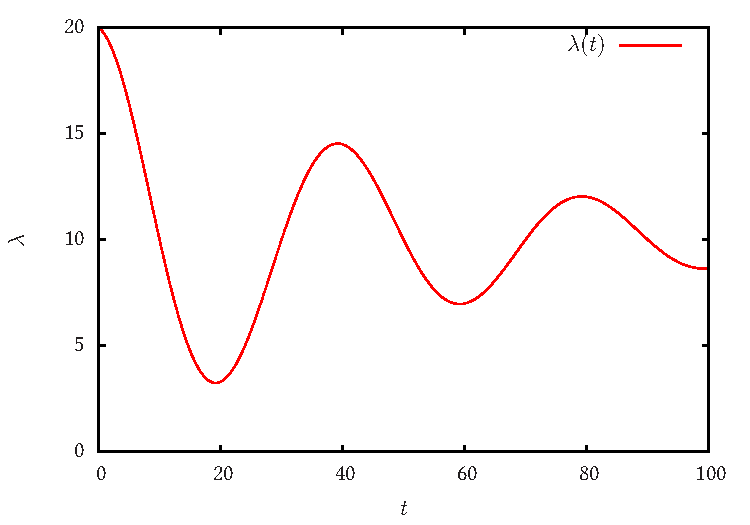
\includegraphics[width=0.5\textwidth]{images/damp}
   }
   \subfloat[]{
   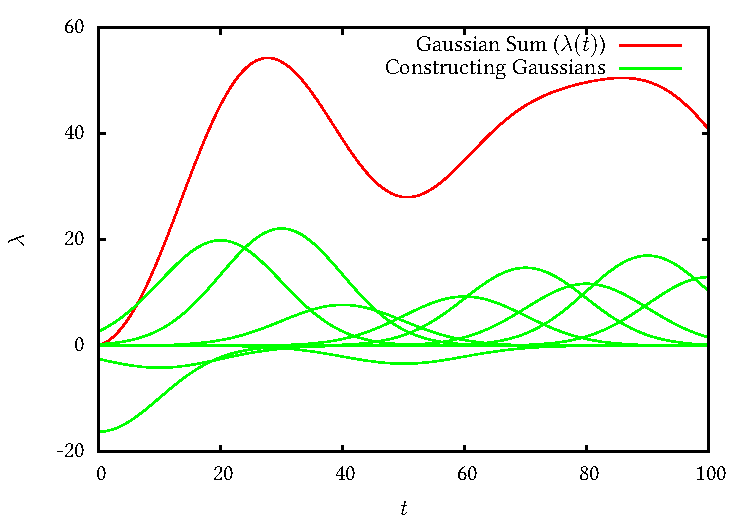
\includegraphics[width=0.5\textwidth]{images/randfunc1}
   }

   \caption{Two examples of function generation capabilities. (a) is generated
   from a damped sine function of the form $e^{-t}\cdot \cos(2\pi t)$. (b) shows
   a randomly generated function where the red function is constructed from the
   green Gaussians with $\Delta t=$ 10, $\mu=$ 10 and shifted so that all points
   are $\geq$ 0.}

   \label{fig:contrib}
   \end{figure}
  The characteristic function of $X$ is modelled as a non-homogeneous Poisson
  process (NHPP) as a continuous function of time, $\lambda(t)$, known as the
  rate function. The system allows the rate function to be specified either by
  providing an expression which is a function of $t$, or by sampling from a
  randomly generated function. Random functions are constructed by uniformly
  distributing $M$ Gaussians across the interval $\left[t_0,T\right]$ in which
  arrival times are to be generated. Each Gaussian $g_i$ is defined by its mean
  $\mu$$_i$, its width $\sigma$$_i$, and its weight $w_i$, which determines its
  height. The means of successive Gaussians are separated by some distance
  $\Delta t$, such that $\mu_{m+1}=\mu_m + \Delta t,\text{ where }
  \mu_0=0$. Greater variation in the functions is introduced by sampling the
  weights $w_i$ from a uniform distribution $U(-1,1)$ and scaling them by some
  multiplier. The value of the randomly generated function at some time $t$ is
  computed by a weighted sum of Gaussians.

  \begin{align}
  \lambda(t) = \sum_{i=0}^M w_i\cdot e^{-(t-\mu_i)^2/2\sigma_i^2}
  \end{align}

  Having defined or constructed $\lambda(t)$, photon arrival times are generated
  from a homogeneous Poisson process (HPP) with constant rate $\lambda$, using
  inverse transform sampling. The waiting time to the next event in a Poisson
  process is \cite{1998art}
  \begin{align}\label{eq:homlambda}
  t=-\frac{1}{\lambda}\log(U)
  \end{align} where $U\sim U(0,1)$. Knowing this, it is possible to generate
  successive events of a HPP for any finite interval, from which events for the
  NHPP can then be extracted by thinning, using Algorithm \ref{alg:seq}. The
  number of events added to the event vector $\Phi$ in any given interval is
  proportional to the value of $\lambda(t)$ in that interval; the probability of
  adding an event is low when $\lambda(t)$ is small, and increases with the
  value of the rate function.

  \begin{algorithm}[H]
  \begin{algorithmic}[1]
  \REQUIRE $\lambda\geq \lambda(t), t_0 \leq t \leq T$
  \STATE $\Phi=\emptyset$, $t=t_0$, $T=\text{interval length}$
  \WHILE{$t<T$}
  \STATE Generate $U_1\sim U(0,1)$
  \STATE $t=t-\frac{1}{\lambda}\ln(U_1)$
  \STATE Generate $U_2\sim U(0,1)$, independent of $U_1$
  \IF{$U_2\leq\frac{\lambda(t)}{\lambda}$}
  \STATE $\Phi \leftarrow t$
  \ENDIF
  \ENDWHILE
  \RETURN $\Phi$
  \end{algorithmic}
  \caption{Generating event times for a NHPP by thinning}
  \label{alg:seq}
  \end{algorithm}
\section{Function Estimation}
\label{sec-3}

  The function estimator subsystem receives input of the event vector $\Phi$, and
  attempts to reconstruct the rate function. As the photons are emitted by a
  truly random process, it is only possible to obtain an estimate of the true
  rate function. In the project, we used two different methods to obtain an
  estimate.
\subsection{Baseline Estimation}
\label{sec-3-1}

   Based on the work of Massey et al.\cite{massey}, we implemented a system to
   estimate the rate function of a set of events using iteratively weighted
   least squares (IWLS). The interval $[t_0,T]$ is split into several bins, each
   represented by the number of events which occur within it. IWLS produces a
   linear estimate of the rate function by an iterative process which minimises
   the sum of squared residuals from an initial estimate of the function.

    \begin{figure}[]
    \centering
    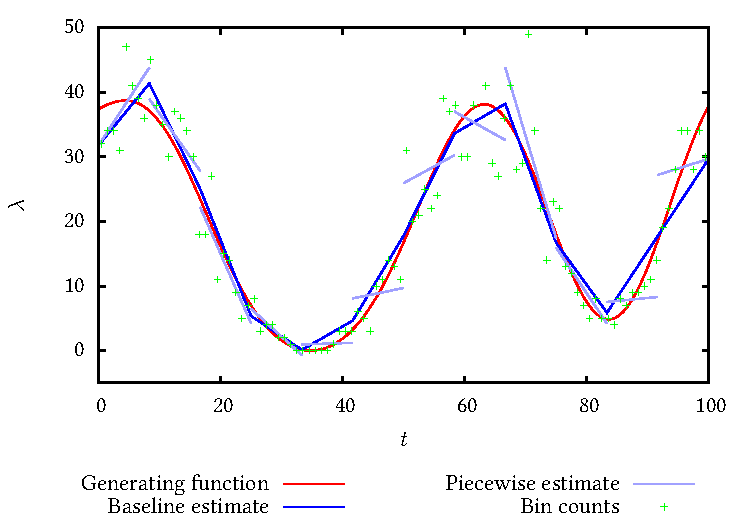
\includegraphics[width=0.8\textwidth]{images/pcbase}

    \caption{A comparison of the baseline and piecewise estimates on the same
    function. Note how the baseline estimate passes through the midpoint of the
    disjoint piecewise estimates at the breakpoints. The estimators used an
    upper limit of 12 sub-intervals, and bins were 1 time unit in length.}

    \label{fig:basecomp}
    \end{figure}

   Linear estimates are not sufficient for representing rate functions, so we
   extended the technique by estimating the rate function in several
   sub-intervals and combining these estimates into a single estimate, rather
   than using a single estimate from the whole interval. Once an estimate for
   the sub-interval has been computed, attempts are made to extend the estimate
   into a short interval after the initial sub-interval. The Poisson probability
   density function (PDF) in Equation \ref{eq:pdf} is used to determine the
   likelihood of obtaining the count $Y_k$ for each bin in the extension
   interval. The likelihood of each bin is required to be above a certain
   threshold. If it is not, the estimate is not extended.
    \begin{equation}
    \label{eq:pdf}
    P(Y_k=x)=\frac{\lambda^xe^{-\lambda}}{x!}
    \end{equation}
    
    This extension of IWLS produces piecewise disjoint estimates of the rate
    function. In order to produce the piecewise continuous functions that we
    require, we adjust the estimate in each sub-interval. We define breakpoints
    as the point in time where one sub-interval ends and another begins. There
    are $R=L-1$ breakpoints $r$, where L is the number of sub-intervals. At each
    breakpoint, the values of the two function estimates $f$ before adjustment
    are computed, and the midpoint $m$ is calculated.

    \begin{equation} 
    m_i = \frac{f_{i}(r_i) + f_{i+1}(r_i)}{2},\quad 0\leq i < R
    \end{equation}

    At the start of the first and end of the last sub-intervals the original
    function value is used as the midpoint. Each sub-interval is now represented
    by a point $p$ at the start and $q$ at the end, each with an $x$ and $y$
    coordinate. With these points, we can recalculate each sub-interval estimate
    $f$ of the form $y=\hat{a}+\hat{b}x$ by replacing $y$ with $p_y$ and $x$
    with $p_x$, and recalculating the gradient $\hat{b}$ and intercept $\hat{a}$
    with
    \begin{align} 
    \hat{b} &= \frac{q_y-p_y}{q_x-p_x}\\
    \hat{a} &= p_y - \hat{b}\cdot p_x 
    \end{align}

    This adjustment produces the desired piecewise continuous function by the
    values of the estimates from the previous and next sub-interval having the
    same value at the breakpoint.
\subsection{Kernel Density (Gaussian) Estimation}
\label{sec-3-2}

    \begin{figure}[h]
    \centering
    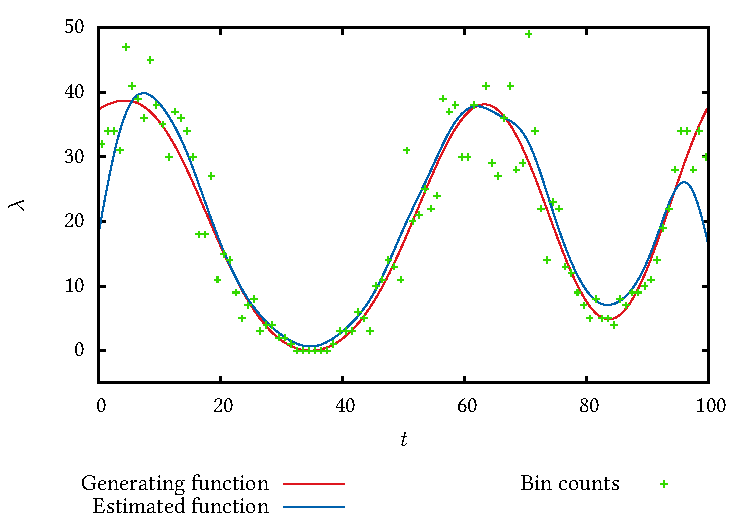
\includegraphics[width=0.8\textwidth]{images/kde}

    \caption{Kernel density estimate of the function from Figure
    \ref{fig:basecomp} showing an example of the smoother functions
    produced. Note the drop-off of the function at the start and end of the
    interval caused by a lack of samples in those areas to allow the result of
    the transform to give an accurate estimate.}

    \label{fig:basecomp}
    \end{figure}

   This method uses \emph{kernels} to estimate the probability density of a
   random variable \cite{cuevas}. Since the photon stream data is generated
   by a source whose variability is defined by some random variable, the event
   times are a sample drawn from the PDF of that variable. We use a Gaussian
   kernel
   \begin{align}
   K(t,\mu)=e^{-(t-\mu)^2/2\sigma^2}
   \end{align}
   to estimate the PDF, centring a kernel at each photon arrival time $\phi_n$ by
   setting $\mu=\phi_n$. The width of the kernel depends on some fixed value
   $\sigma$. We perform a Gauss transform on the $N$ kernels, finding the
   contribution of all the kernels at $M$ points in time, from which we get an
   estimate $\hat{\lambda}(t)$ of the characteristic function.

   \begin{align}
   \hat{\lambda}(t_i) = \sum_{j=1}^N K(t_i,\mu_j), \quad i=1,\dots,M
   \end{align}

   Using a larger $M$ gives a higher resolution. Depending on the value of
   $\sigma$ used, $\hat{\lambda}(t)$ will be some multiple of the actual
   function $\lambda(t)$. Thus, the final step is to normalise
   $\hat{\lambda}(t)$. We split the stream data into $B$ bins with midpoints $b$
   and calculate the bin count $x$ for each. We start with the normalisation
   constant $\eta$ at a low value, and gradually increase it to some threshold,
   finding

   \begin{equation}\label{eq:normcalc}
   \sum_{i=1}^B
   \log\left(\frac{\phi^xe^{-\phi}}{x!}\right), \quad \phi=\eta\cdot\hat{\lambda}(b_i)
   \end{equation}

   for each value of $\eta$. The value of $\eta$ which maximises this sum of log
   Poisson PDFs is used to normalise $\hat{\lambda}(t)$ in subsequent
   computations.
\section{Time Delay Estimation}
\label{sec-4}

  Once we are able to estimate the characteristic function of photon streams, we
  can use these estimates to compute an estimate of the time delay between two
  streams. If the two streams come from the same source, then they should have
  the same characteristic function, but delayed by some value $\Delta$. Our
  estimates of the characteristic function will differ for both streams due to
  the fact that the number of photon arrivals in each bin will be different for
  each stream, but each should look similar. In this section we present two
  methods for estimating the time delay between a pair of streams based on their
  function estimates.

  Both of the estimators work by starting $\Delta$ at $-\Delta_{\text{max}}$,
  and increment it by some step until $+\Delta_{\text{max}}$ is reached, using a
  metric to evaluate how good the estimate is with that value. Estimates are
  computed based on data in the interval
  $T_{\text{est}}=[t_0+\Delta_{\text{max}}, T-\Delta_{\text{max}}]$, where
  $\Delta_{\text{max}}<T$. This constraint on $T_{\text{est}}$ means that there
  is no need to normalise the likelihood of matches due to differing interval
  lengths.

  In the approximation, $t$ is incremented by some finite step for each
  successive value. As with the previous estimator, the estimate is made in two
  stages, first with a coarse pass over the values of delta to compute an
  initial estimate, and then a finer second pass around the first estimated
  value in order to refine the estimate.
\subsection{Area Method}
\label{sec-4-1}

   \begin{figure}[]
   \subfloat[High area ($\Delta=$ 5)]{
   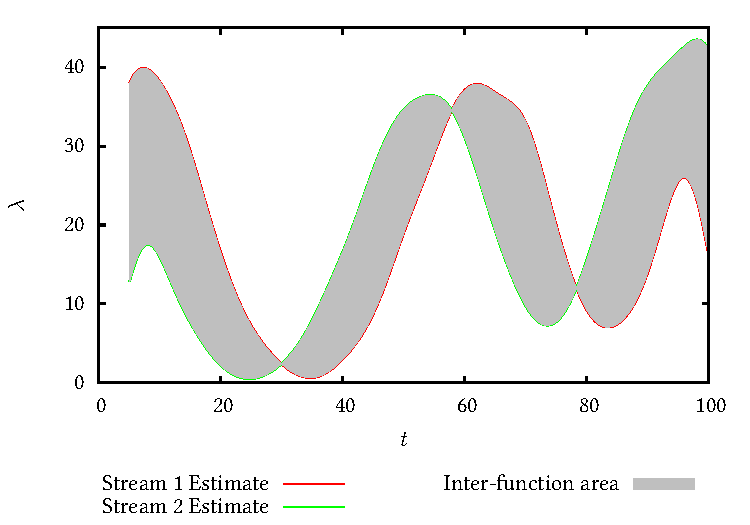
\includegraphics[width=0.5\textwidth]{images/area_gauss_large}
   %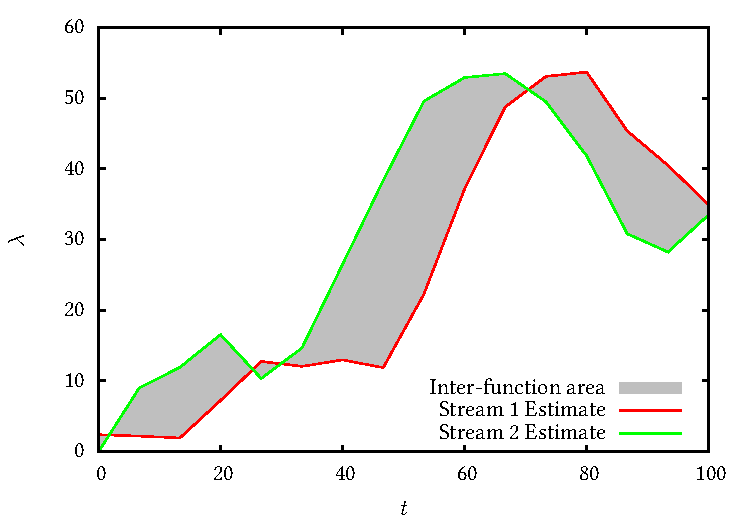
\includegraphics{normarea}
   }
   \subfloat[Low area ($\Delta=$ 15.1)]{
   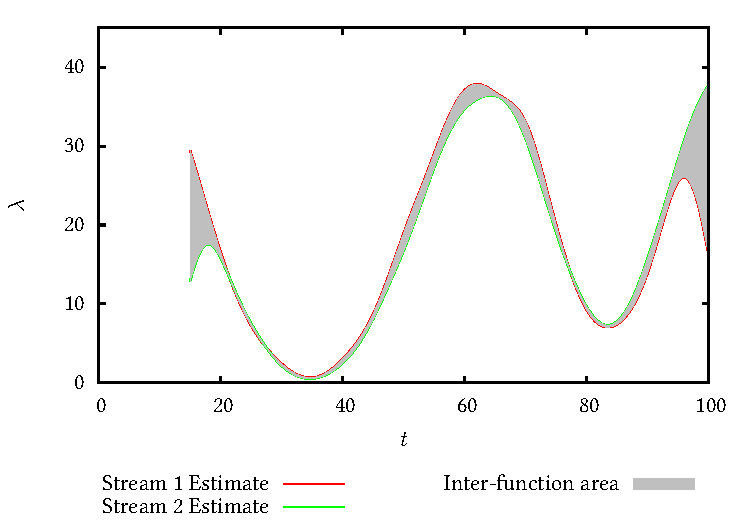
\includegraphics[width=0.5\textwidth]{images/area_gauss_small}
   %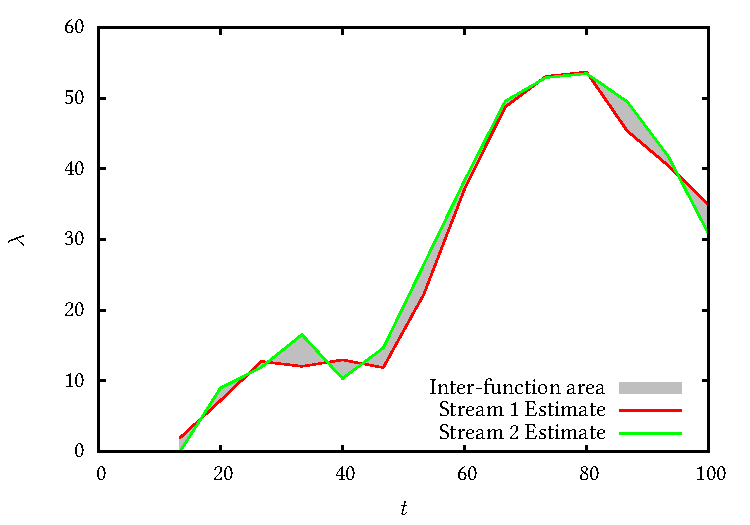
\includegraphics{shiftarea}
   }

   \caption{An illustration of the idea behind the area method. In (a), the
   applied shift results in a large area between the functions. In (b), the
   shift is very close to the actual time delay ($\Delta=15$), and the resulting
   area is much smaller than (a), indicating that the shift in (b) is a better
   estimate.}

   \label{fig:areamethod}
   \end{figure}
   The first method uses a very simple metric to estimate the time delay. Taking
   the two function estimates, we attempt to match them up so that they ``fit
   together'' best, as in Figure \ref{fig:areamethod}. The goodness of fit
   between two functions $\hat{\lambda}_1$ and $\hat{\lambda}_2$ is defined by
   the area between them, calculated by
   \begin{align}
   \begin{split}
   d(\hat{\lambda}_1,\hat{\lambda}_2)&=\int(\hat{\lambda}_1(t)-\hat{\lambda}_2(t+\Delta))^2\,dt\\
   &\approx\frac{1}{N}\sum_{i=1}^N(\hat{\lambda}_1(t)-\hat{\lambda}_2(t+\Delta))^2
   \end{split}
   \end{align}
   for each value of $\Delta$. Our estimate of $\Delta$ is set to the value at
   which $d(\hat{\lambda}_1,\hat{\lambda}_2)$ is minimised. Rather than using an
   integral to get the exact area between the functions, we use a less
   computationally expensive discrete approximation.
\subsection{PDF Method}
\label{sec-4-2}

   The second method of estimation uses probability density functions. As
   before, we guess a value of $\Delta$ between $-\Delta_{\text{max}}$ and
   $+\Delta_{\text{max}}$ and shift $\hat{\lambda}_2$ by that amount. However,
   we know that there must be a single characteristic function, and we want to
   see how well our estimate of that matches the bin counts in each stream. We
   make an ``average'' function $\bar{\lambda}$ by combining the two function
   estimates we have, $\hat{\lambda}_1$ and $\hat{\lambda}_2$ (which is shifted
   by $\Delta$).
   \begin{equation}
   \bar{\lambda}(t)=\frac{\hat{\lambda}_1(t)+\hat{\lambda}_2(t+\Delta)}{2}
   \end{equation}
   The point on $\bar{\lambda}$ at time $t$ is the midpoint between the values of
   the two estimates at that time. Once we have $\bar{\lambda}$, we can assign some
   score to the current estimate of the value of $\Delta$.

   \begin{align}
   \begin{split}
   \log P(S_A,S_B\mid\bar{\lambda}(t))=\sum_{t=\Delta_{\text{max}}}^{T-\Delta_{\text{max}}}&\log P(S_A(t)\mid \bar{\lambda}(t))\\
   &+ \log P(S_B(t+\Delta)\mid \bar{\lambda}(t))\\
   \label{eq:cfuncprob}
   \end{split}
   \end{align}
   
   Using \eqref{eq:cfuncprob}, we calculate the probability that the function
   $\bar{\lambda}$ is the characteristic function of the two streams $S_A$ and
   $S_B$. The streams are split into bins, and the log probability of the number
   of events in each bin given the value of $\lambda$ calculated for that bin is
   computed and summed over all bins, using \eqref{eq:normcalc}.

   Since we are considering a number of events occurring in a given interval, we
   must consider the value of $\lambda$ for the same interval. In order to do
   this, we use a discrete approximation of integrating $\lambda(t)$ over the
   interval.

   \begin{align}
   \lambda_{a,b}&=\int_a^b\lambda(t)\,dt
   \end{align}
   
   The estimated value of $\Delta$ is set to the value which has the highest sum of log
   probabilities.

   \begin{figure}[]
   \subfloat[Estimate $\lambda(t)$ for each stream based on bin data.]{
   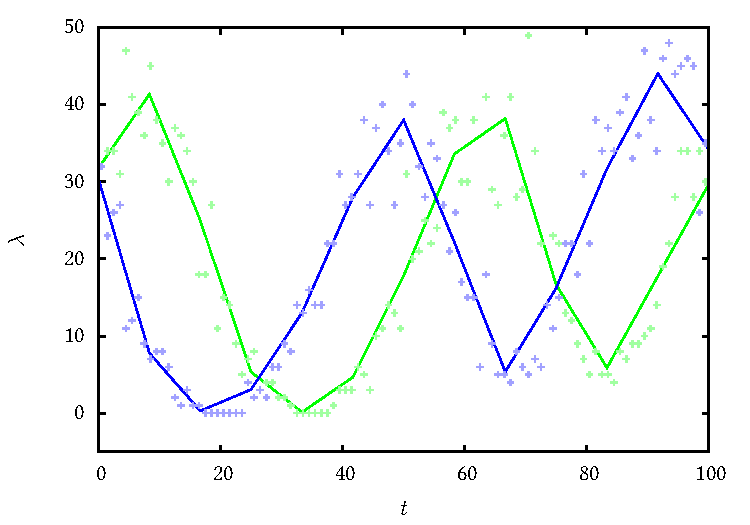
\includegraphics[width=0.5\textwidth]{images/twofunc_base}
   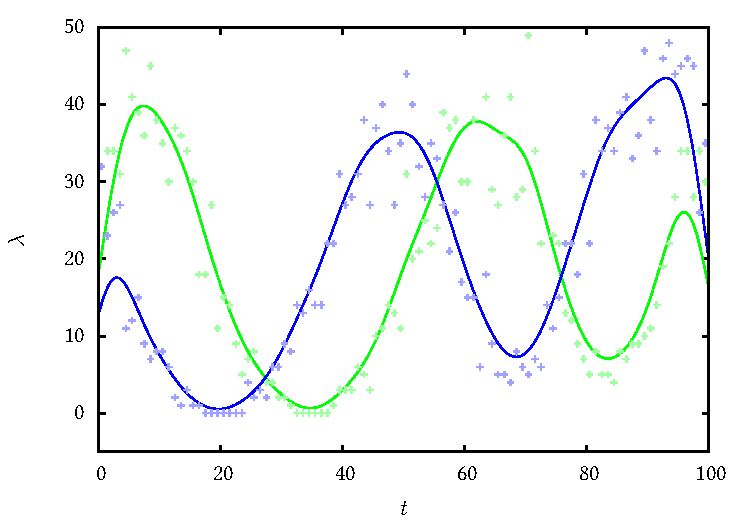
\includegraphics[width=0.5\textwidth]{images/twofunc_gauss}
   }\\
   \subfloat[Run the time delay estimator and shift the second (blue) function according to the estimate of $\Delta$.]{
   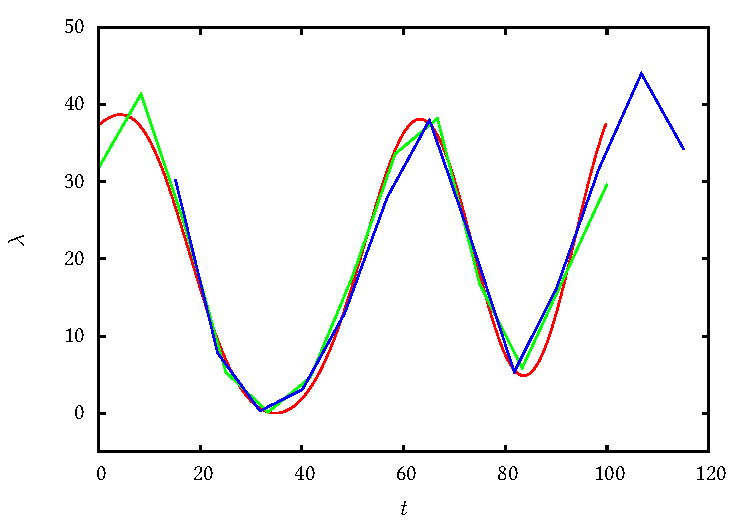
\includegraphics[width=0.5\textwidth]{images/shift_base}
   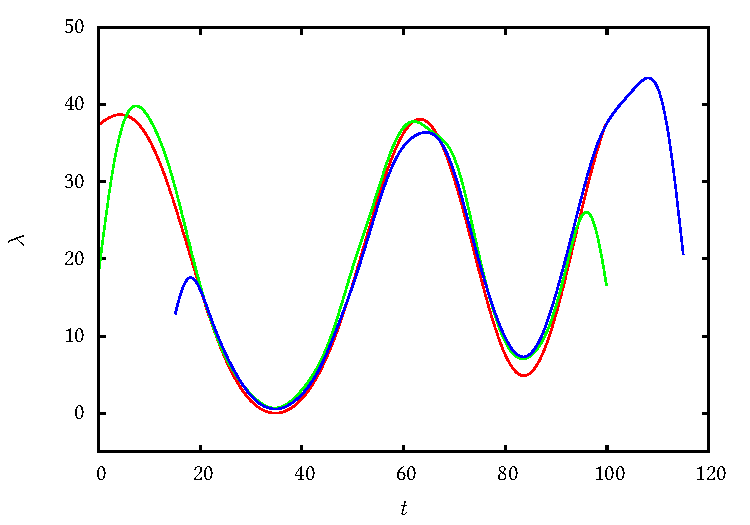
\includegraphics[width=0.5\textwidth]{images/shift_gauss}
   }\\
   \subfloat[Combine the two function estimates to create a final estimate (black).]{
   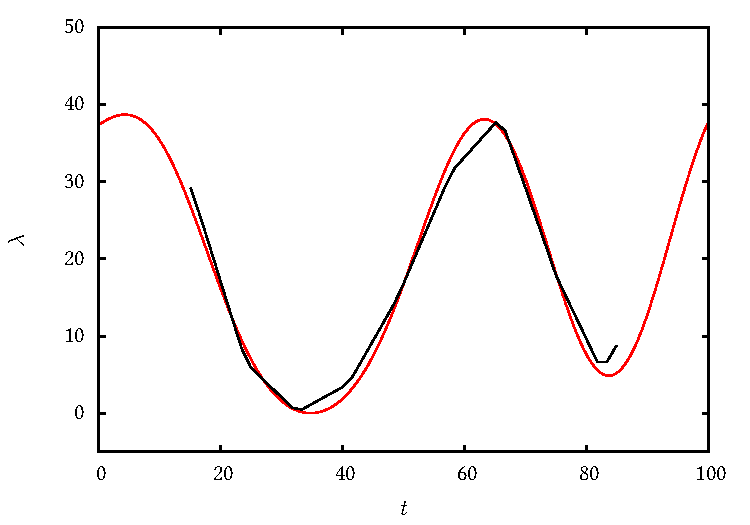
\includegraphics[width=0.5\textwidth]{images/comb_base}
   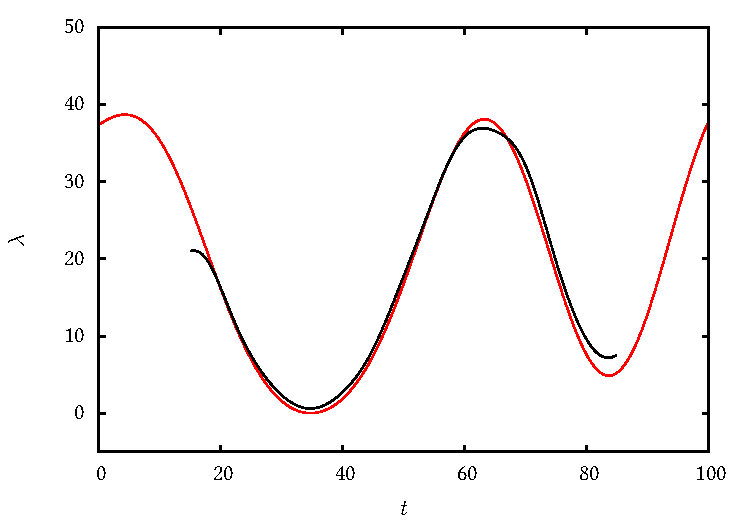
\includegraphics[width=0.5\textwidth]{images/comb_gauss}
   }

   \caption{An example of the estimation process using two different
   techniques. Left column shows baseline method, right column Gaussian. The
   estimated value of $\Delta$ was 15.1 for both estimators, found using the PDF
   method. The actual value of $\Delta$ was 15. Points in (a) represent bin
   counts for the function of the same colour. The red line in (b) and (c)
   indicates the actual function, black is the final estimate. Estimated
   functions are only combined in the interval in which they both have values.}

   \label{fig:finest}
   \end{figure}
\section{Experimental Results}
\label{sec-5}

  The four possible method combinations were compared in four sets of
  experiments. 100 time units of Photon stream data was generated from sine
  functions of the form $y=a-b\sin(\alpha t)$ in the first set of two
  experiments, and from randomly generated functions in the second set. In both
  cases the $\alpha$ parameter defined the variability of the function. The
  experiments tested performance on functions generated with several different
  $\alpha$ values. Multiple photon streams were generated from each function to
  obtain a larger statistical sample. The sine function experiments used 25
  independently generated stream pairs for the first, and 10 for the
  second. Random function experiments used 5 pairs for each of the 5 functions
  tested.
    \begin{figure}[]
    \subfloat[Baseline area]{
    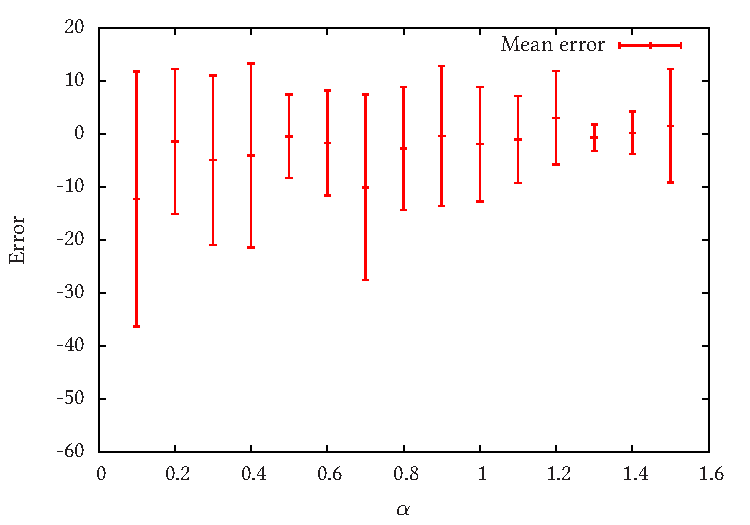
\includegraphics[width=0.5\textwidth]{images/baseline_area_morerand}
    }
    \subfloat[Baseline PDF]{
    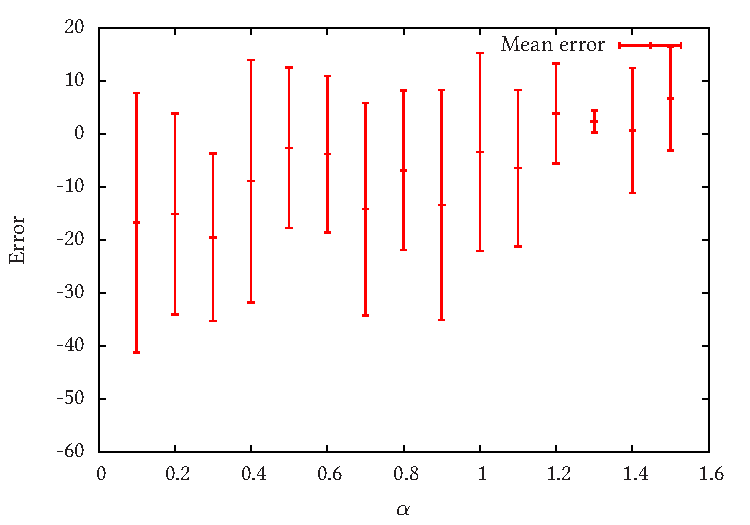
\includegraphics[width=0.5\textwidth]{images/baseline_pmf_morerand}
    }\\
    \subfloat[Gaussian area]{
    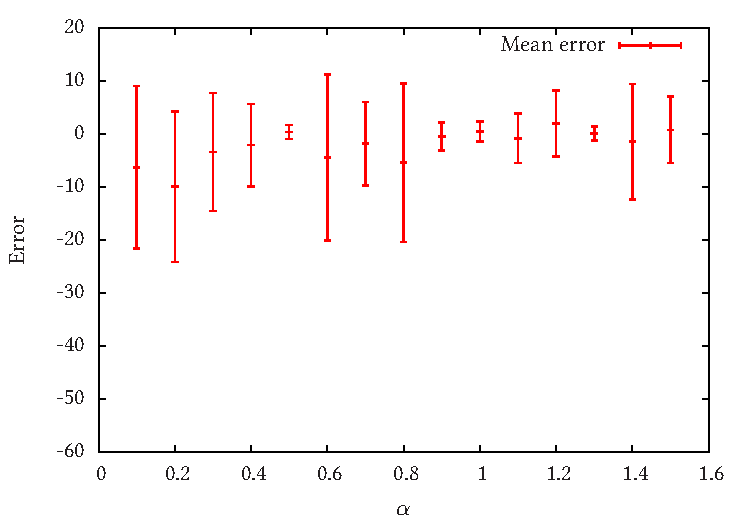
\includegraphics[width=0.5\textwidth]{images/gaussian_area_morerand}
    }
    \subfloat[Gaussian PDF]{
    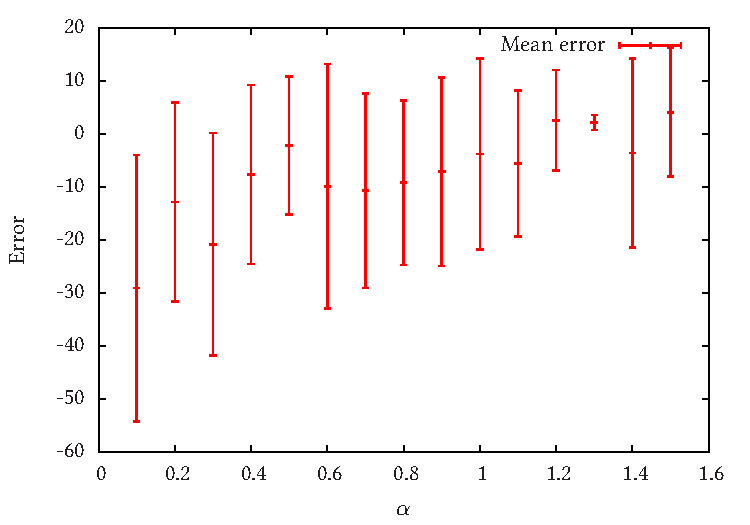
\includegraphics[width=0.5\textwidth]{images/gaussian_pmf_morerand}
    }

    \caption{Grand mean of error on estimates over 5 functions for each value of
    $\alpha$ for the second set of random function experiments. Error bars show
    standard deviation. The error and standard deviation when using the area
    method appears much lower than that of the PDF method, and the Gaussian area
    method in particular seems to produce much better estimates than others.}

    \label{fig:moreranderror}
    \end{figure}
  \begin{table}[]

  \begin{center}
  \centerline{
  \begin{tabular}{r|cccccc}
  $\alpha$  &  Baseline area        &  Baseline PDF         &  Gaussian area        &  Gaussian PDF          \\
  \hline
  0.1  &  2.668 $\pm$ 24.011   &  -1.808 $\pm$ 24.508  &  8.656 $\pm$ 15.301   &  -14.152 $\pm$ 25.117  \\
  0.3  &  9.976 $\pm$ 15.983   &  -4.576 $\pm$ 15.793  &  11.528 $\pm$ 11.16   &  -5.872 $\pm$ 20.965   \\
  0.5  &  14.508 $\pm$ 7.9035  &  12.312 $\pm$ 15.138  &  15.316 $\pm$ 1.3203  &  12.732 $\pm$ 12.987   \\
  0.7  &  4.88 $\pm$ 17.486    &  0.74 $\pm$ 20.025    &  13.096 $\pm$ 7.8901  &  4.236 $\pm$ 18.376    \\
  0.9  &  14.568 $\pm$ 13.218  &  1.524 $\pm$ 21.66    &  14.488 $\pm$ 2.6585  &  7.8 $\pm$ 17.765      \\
  1.1  &  13.9 $\pm$ 8.1991    &  8.496 $\pm$ 14.743   &  14.1 $\pm$ 4.6522    &  9.348 $\pm$ 13.755    \\
  1.3  &  14.228 $\pm$ 2.5246  &  17.264 $\pm$ 2.0459  &  15.028 $\pm$ 1.3014  &  17.096 $\pm$ 1.4202   \\
  1.5  &  16.46 $\pm$ 10.726   &  21.592 $\pm$ 9.7962  &  15.724 $\pm$ 6.2363  &  19.004 $\pm$ 12.125   \\
  \end{tabular}
  }
  \end{center} 

\caption{A selection of results from the second set of random function
  experiments. Values shown are calculated by aggregating estimate data from 5
  functions with 5 estimates for each $\alpha$ value. The actual time delay
  is 15. ($\mu\pm\sigma,\,n=$ 25)}
\end{table}   
\begin{figure}[]
\subfloat[$\alpha_{\text{sine}}=0.005$]{
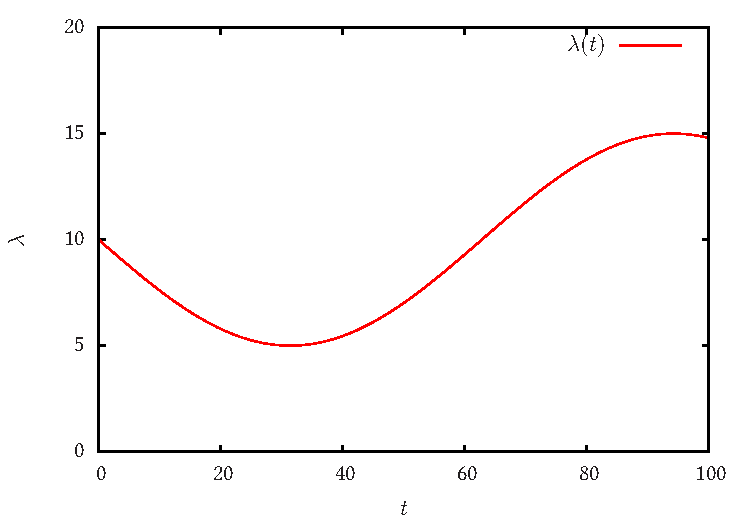
\includegraphics[width=0.5\textwidth]{images/prelim_sine_005}
}
\subfloat[$\alpha_{\text{gauss}}=0.4$]{
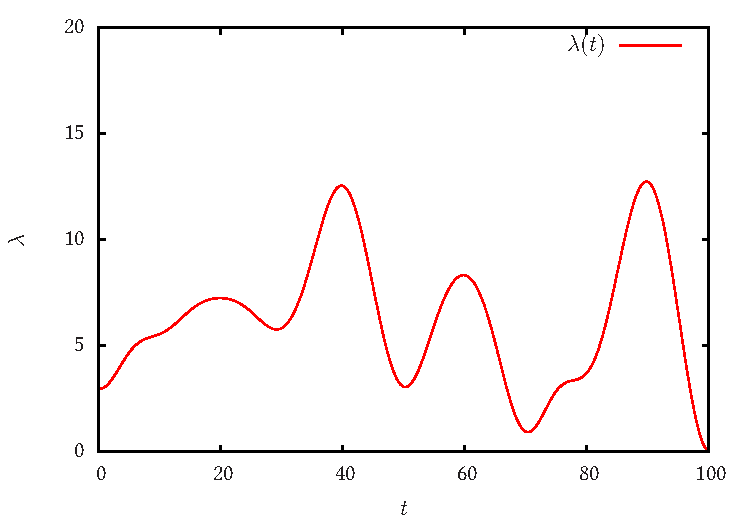
\includegraphics[width=0.5\textwidth]{images/randfunc_04}
}

\subfloat[$\alpha=_{\text{sine}}0.06$]{
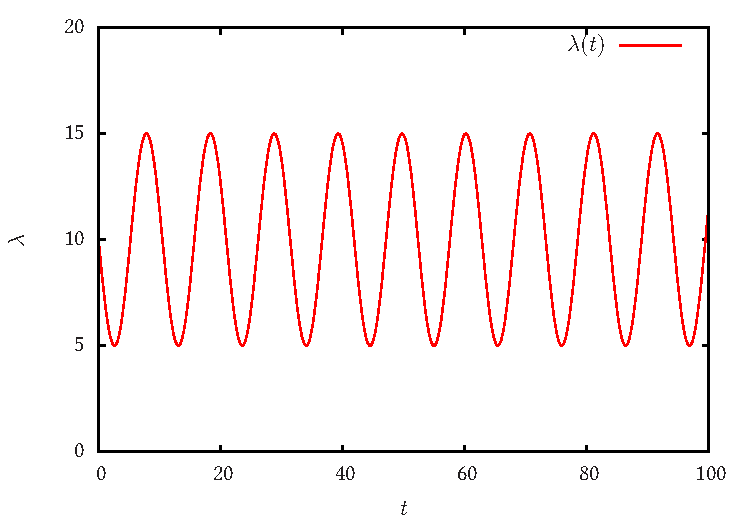
\includegraphics[width=0.5\textwidth]{images/prelim_sine_06}
}
\subfloat[$\alpha=_{\text{gauss}}3$]{
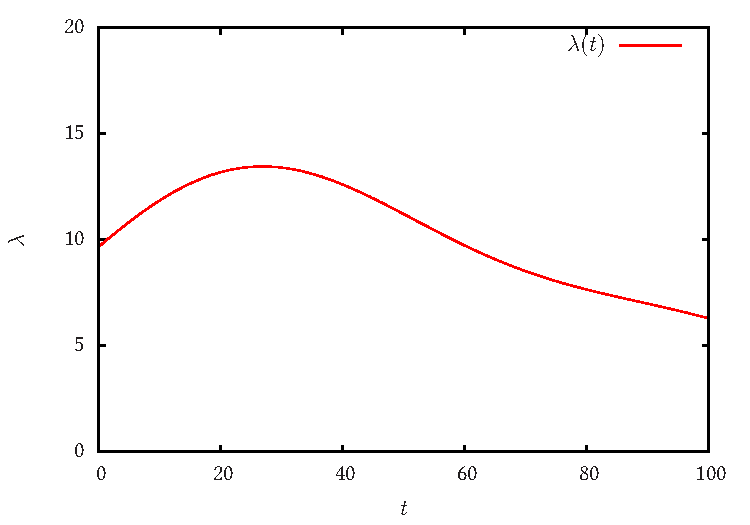
\includegraphics[width=0.5\textwidth]{images/randfunc_3}
}

\caption{A range of different functions was used during the experiments. The
parameter $\alpha$ controlled the smoothness of the functions. In the sine
function experiments, lower values of $\alpha$ resulted in a higher oscillation
frequency (a and c). In the random function experiments, the width of Gaussians
used to construct the functions was determined by $\sigma=\alpha\cdot\Delta t$,
where $\Delta t$ is the separation distance between successive
Gaussians(b and d).}

\end{figure}
  The first stage of each experiment found optimum parameter settings for each
  function in the experimental data set using model selection. The kernel
  density and baseline estimators were used to find $\hat{\lambda}(t)$ from
  stream data where 4 time units of stream data were withheld every 15 time
  units. The number of events in each bin in withheld sub-intervals was
  retrieved from the stream and compared to the value of $\hat{\lambda}(t)$ at
  the midpoint of that bin using the log Poisson PDF. The sum of log PDF values
  over all the sub-intervals was used to represent the parameter set's
  generalisation ability. The set with the highest value was used in the second
  stage of the experiment, where the time delay for a pair of streams was
  estimated using both the area and the PDF methods. This resulted in 4
  estimates of the time delay, one from each combination of function estimator
  and time delay estimator.

  Paired and single-sample t-tests were applied to the resulting estimates to
  check for any significant difference in the performance of the method
  combinations, but there was no indication of any significance.
\section{Conclusion}
\label{sec-6}

  In this summary, we provided an overview of the concepts behind our time delay
  estimation methods for paired photon streams. The Gaussian area estimator
  appears to perform best, and our experimental results indicate directions for
  further work. A fast Gauss transform implementation would improve computation
  time for the kernel density estimator. Hierarchical search to find the maximum
  of the PDF at the baseline estimator breakpoints would improve the quality of
  estimates. Further improvements could come from an investigation into
  techniques to deal with highly symmetric or repeating functions such as sine
  waves.

\printbibliography

\end{document}